\documentclass[SingleSpace,12pt,Proceedings]{Serre_ASCE}

\usepackage[dvips]{graphicx}
\usepackage{amsmath}
\usepackage{amsfonts}
\usepackage{amssymb}
\usepackage[pdf]{pstricks}
\usepackage{psfrag}
\usepackage{pifont}
\usepackage{epstopdf}
%\usepackage{topcapt}
\usepackage{lscape}
\usepackage{amsthm}
\usepackage{url}
\usepackage{pifont}
\usepackage{geometry}
\usepackage{fleqn}
\usepackage{txfonts}
\usepackage{wasysym}
\usepackage{lineno}
\usepackage{enumerate}
\usepackage{url}
\usepackage{times}
\usepackage{subfigure}
\usepackage{graphicx}
\usepackage{longtable}
%\usepackage{citeref}
\usepackage[skip=0pt]{caption}

% TIME ON EVERY PAGE AS WELL AS THE FILE NAME
\usepackage{fancyhdr}
\usepackage{currfile}
\usepackage[us,12hr]{datetime} % `us' makes \today behave as usual in TeX/LaTeX
\fancypagestyle{plain}{
\fancyhf{}
\rfoot{\small Draft Paper \\ File Name: {\currfilename} \\ Date: {\ddmmyyyydate\today} at \currenttime}
\lfoot{Page \thepage}
\renewcommand{\headrulewidth}{0pt}}
\pagestyle{plain}

\begin{document}

\title{Behaviour of the Dam-Break Problem for the Serre Equations}

\author{
Jordan~Pitt,%
\thanks{Mathematical Sciences Institute, Australian National University, Canberra, ACT 0200, Australia, E-mail: Jordan.Pitt@anu.edu.au. The work undertaken by the first author was supported financially by an Australian National University Scholarship.}
\\
Christopher~Zoppou,\footnotemark[1]%
%
% Adding a second author with the same affiliation (still using \thanks):
\\
Stephen~G.~Roberts,\footnotemark[1]
}

\maketitle

\begin{abstract}

\end{abstract}

\KeyWords{dispersive waves, conservation laws, Serre equation, finite volume method, finite difference method}

\linenumbers

%--------------------------------------------------------------------------------
\section{Introduction} \label{intro} 

%--------------------------------------------------------------------------------
\section{Serre Equations}
\label{section:Serre Equations}
The Serre equations can derived as an approximation to the full Euler equations by depth integration similar to \cite{Su-Gardener-1969-536}. They can also be seen as an asymptotic expansion to the Euler equations as well \cite{Bonneton-Lannes-2009-16601}. The former is more consistent with the perspective from which numerical methods will be developed while the latter indicates the appropriate regions in which to use these equations as a model for fluid flow.
\begin{figure}[htb]
\begin{center}
\includegraphics[width=7.0cm]{one-dimensional-axis_Serre.eps}
\end{center}
\caption{The notation used for one-dimensional flow governed by the Serre equation.}
\label{fig:Notation}
\end{figure}
The set up of the scenario under which the Serre approximation is made consists of a two dimensional $\textbf{x} = (x,z)$ fluid over a bottom topography as in Figure \ref{fig:Notation} acting under gravity. Consider a fluid particle at depth  $\xi(\textbf{x},t) = h(x,t) + z_b(x) - z$ below the water surface, see Figure \ref{fig:Notation}. Where the water depth is $h(x,t)$ and $z_b(x)$ is the bed elevation. The fluid particle is subject to the pressure, $p(\textbf{x},t)$ and  gravitational acceleration, $\textbf{g} = (0,g)^T$ and has a velocity $\textbf{u} = (u(\textbf{x},t),w(\textbf{x},t))$,  where $u(\textbf{x},t)$ is the velocity in the $x$-coordinate and $w(\textbf{x},t)$ is the velocity in the $z$-coordinate and $t$ is time. Assuming that $z_b(x)$ is constant the Serre equations read \cite{Guyenne-etal-2014-169}
\begin{linenomath*}
\begin{subequations}\label{eq:Serre_nonconservative_form}
\begin{gather}
\dfrac{\partial h}{\partial t} + \dfrac{\partial (\bar{u}h)}{\partial x} = 0
\label{eq:Serre_continuity}
\end{gather}
\begin{gather}
\underbrace{\underbrace{\dfrac{\partial (\bar{u}h)}{\partial t} + \dfrac{\partial}{\partial x} \left ( \bar{u}^2h + \dfrac{gh^2}{2}\right )}_{\text{Shallow Water Wave Equations}} + \underbrace{\dfrac{\partial}{\partial x} \left (  \dfrac{h^3}{3} \left [ \dfrac{\partial \bar{u} }{\partial x} \dfrac{\partial \bar{u}}{\partial x} - \bar{u} \dfrac{\partial^2 \bar{u}}{\partial x^2}  - \dfrac{\partial^2 \bar{u}}{\partial x \partial t}\right ] \right )}_{\text{Dispersion Terms}} = 0.}_{\text{Serre Equations}}
\label{eq:Serre_momentum}
\end{gather}
\end{subequations}
\end{linenomath*}
Where $\bar{u}$ means the average of $u$ over the depth of water. 
%--------------------------------------------------------------------------------
\section{Direct Numerical Methods} 
\label{sec:DirNumMet}
%--------------------------------------------------------------------------------
The presence of the mixed spatial temporal derivatives in the momentum equation \eqref{eq:Serre_momentum} makes the Serre equations difficult to solve directly with standard numerical methods. A naive way to avoid this is to approximate \eqref{eq:Serre_momentum} by finite differences and the results of this are presented here. To facilitate this a uniform grid in space will be used with $\Delta x  = x_{i+1} - x_i$ for all $i$ and quantities evaluated at these grid points will be denoted by subscripts for example $h_i = h(x_i)$. The grid in time will be denoted by superscripts for example $h^n = h(t^n)$, noting that $h^n$ is a function in space. 
\subsection{Finite Difference Appximation to Conservation of Momentum Equation} 
In [][Zoppou thesis/my work] it was demonstrated that an efficient numerical scheme for the Serre equations must be at least second-order accurate thus the derivatives in \eqref{eq:Serre_momentum} will be approximated by second-order finite differences. Firstly \eqref{eq:Serre_momentum} must be expanded, making use of \eqref{eq:Serre_continuity} one obtains
\begin{linenomath*}
\begin{subequations}
\begin{gather}
h\dfrac{\partial u}{\partial t} + X - h^2\frac{\partial^2 u}{\partial x \partial t} - \frac{h^3}{3}\frac{\partial^3 u}{\partial x^2 \partial t}  =0 
\label{eq:expandedu}
\end{gather}
where $X$ contains only spatial derivatives and is
\begin{gather}
X = uh\frac{\partial u}{\partial x} + gh\frac{\partial h}{\partial x} + h^2\frac{\partial u}{\partial x}\frac{\partial u}{\partial x} + \frac{h^3}{3}\frac{\partial u}{\partial x}\frac{\partial^2 u}{\partial x^2} - h^2u\frac{\partial^2 u}{\partial x^2}- \frac{h^3}{3}u\frac{\partial^3 u}{\partial x^3}
\end{gather}
\end{subequations}
\end{linenomath*}
where the bar over $u$ has been dropped to simplify notation. Then taking second-order centred finite difference approximation to the time derivatives for \eqref{eq:expandedu} gives
\begin{linenomath*}
\begin{gather*}
h^{n}\dfrac{u^{n+1} - u^{n-1}}{2 \Delta t} + X^{n} - \left(h^{n}\right)^2\frac{ \left(\frac{\partial u}{\partial x}\right)^{n+1} - \left(\frac{\partial u}{\partial x}\right)^{n-1} }{2 \Delta t} - \frac{\left(h^{n}\right)^3}{3}\frac{ \left(\frac{\partial^2 u}{\partial x^2}\right)^{n+1} - \left(\frac{\partial^2 u}{\partial x^2}\right)^{n-1} }{2 \Delta t}  =0, 
\label{eq:expandedutdisc}
\end{gather*}
\end{linenomath*}
\begin{linenomath*}
\begin{gather*}
h^{n} \left(u^{n+1} - u^{n-1}\right) + 2\Delta tX^{n} - \left(h^{n}\right)^2 \left(\left(\frac{\partial u}{\partial x}\right)^{n+1} - \left(\frac{\partial u}{\partial x}\right)^{n-1}\right) - \frac{\left(h^{n}\right)^3}{3}\left(\left(\frac{\partial^2 u}{\partial x^2}\right)^{n+1} - \left(\frac{\partial^2 u}{\partial x^2}\right)^{n-1} \right)  =0. 
\label{eq:expandedutdisc1}
\end{gather*}
\end{linenomath*}

%\begin{linenomath*}
%\begin{gather*}
%h^{n}u^{n+1} - \left(h^{n}\right)^2 \left(\frac{\partial u}{\partial x}\right)^{n+1} - \frac{\left(h^{n}\right)^3}{3}\left(\frac{\partial^2 u}{\partial x^2}\right)^{n+1}  + 2\Delta tX^{n} - h^{n}u^{n-1} + \left(h^{n}\right)^2\left(\frac{\partial u}{\partial x}\right)^{n-1} + \frac{\left(h^{n}\right)^3}{3}\left(\frac{\partial^2 u}{\partial x^2}\right)^{n-1}   =0 
%\label{eq:expandedutdisc2}
%\end{gather*}
%\end{linenomath*}
Introducing
\begin{linenomath*}
\begin{gather*}
Y^n = 2\Delta tX^{n} - h^{n}u^{n-1} + \left(h^{n}\right)^2\left(\frac{\partial u}{\partial x}\right)^{n-1} + \frac{\left(h^{n}\right)^3}{3}\left(\frac{\partial^2 u}{\partial x^2}\right)^{n-1}
\label{eq:expandfactor Xp}
\end{gather*}
\end{linenomath*}
and rearranging results in
\begin{linenomath*}
\begin{gather*}
h^{n}u^{n+1} - \left(h^{n}\right)^2 \left(\frac{\partial u}{\partial x}\right)^{n+1} - \frac{\left(h^{n}\right)^3}{3}\left(\frac{\partial^2 u}{\partial x^2}\right)^{n+1}  + Y^n   =0 . 
\label{eq:expandedutdisc2}
\end{gather*}
\end{linenomath*}

Taking second-order approximations to the spatial derivatives and evaluating the quantities at the correct locations gives
\begin{linenomath*}
\begin{gather}
h^{n}_iu^{n+1}_i - \left(h^{n}_i\right)^2 \left(\frac{u^{n+1}_{i+1} -u^{n+1}_{i-1} }{2 \Delta x}\right) - \frac{\left(h^{n}_i\right)^3}{3}\left(\frac{u^{n+1}_{i+1} - 2u^{n+1}_{i} + u^{n+1}_{i-1} }{\Delta x^2}\right) = - Y^n_i 
\label{eq:expandedutdisc3}
\end{gather}
\end{linenomath*}
This can be rearranged into a tri-diagonal matrix that updates $u$ given its current and previous values. So that
\begin{linenomath*}
\begin{gather}
\left[\begin{array}{c}
 u^{n+1}_0 \\
 \vdots \\
 u^{n+1}_m \end{array}\right]
 = A^{-1} \left[\begin{array}{c}
  -Y^n_0 \\
  \vdots \\
  -Y^n_m \end{array}\right] =: \mathcal{G}_u\left(\boldsymbol{u}^n,\boldsymbol{h}^n, \boldsymbol{u}^{n-1},\boldsymbol{h}^{n-1}, \Delta x, \Delta t \right).
\label{eq:FDcentforu}
\end{gather}
\end{linenomath*}
Where
\begin{linenomath*}
\begin{gather*}
A =
\left[\begin{array}{ccccccccc}
 b_0 & c_0 &  & & & &  \\
 a_0 & b_1 & c_1 &  & & & \\
  & a_1 & b_2 & c_2 &  & &   \\
  &  &\ddots &\ddots &\ddots & & \\
  &  &  & a_{m-3} & b_{m-2} & c_{m-2} & \\
  &  &  &  & a_{m-2} & b_{m-1} & c_{m-1} \\
  &  &  & &  & a_{m-1} & b_{m}\\
  \end{array}\right]
\end{gather*}
\end{linenomath*}
with
\begin{subequations}
\begin{gather}
a_{i-1} = \frac{\left(h^n_i\right)^2}{2\Delta x}\frac{h^n_{i+1} - h^n_{i-1}}{2\Delta x} - \frac{\left(h^n_i\right)^3}{3 \Delta x^2}  ,
\label{eq:utriAa}
\end{gather}
\begin{gather}
b_i = h^n_i + \frac{2 h^n_i}{3 \Delta x^2}
\label{eq:utriAb}
\end{gather}
and
\begin{gather}
c_i = -\frac{\left(h^n_i\right)^2}{2\Delta x}\frac{h^n_{i+1} - h^n_{i-1}}{2\Delta x} - \frac{\left(h^n_i\right)^3}{3 \Delta x^2}.
\label{eq:utriAc}
\end{gather}
\end{subequations}
Lastly for completeness the final expression for $Y^n_i$ is given by
\begin{linenomath*}
\begin{gather}
\begin{split}
Y^n_i &= 2\Delta t \Bigg[u^n_ih^n_i \frac{u^{n}_{i+1} - u^{n}_{i-1}}{2\Delta x} + gh^n_i\frac{h^{n-1}_{i+1} - h^{n-1}_{i-1}}{2\Delta x} + \left(h^n_i\right)^2 \left(\frac{u^{n-1}_{i+1} - u^{n-1}_{i-1}}{2\Delta x} \right)^2 \\ &+ \frac{\left(h^n_i\right)^3}{3}\frac{u^{n}_{i+1} - u^{n}_{i-1}}{2\Delta x}\frac{u^{n}_{i+1} -2u^{n}_{i}   + u^{n}_{i-1}}{\Delta x^2} - \left(h^n_i\right)^2u^n_i\frac{u^{n}_{i+1} -2u^{n}_{i} + u^{n}_{i-1}}{\Delta x^2}  \\  &- \frac{\left(h^n_i\right)^3}{3}u^n_i\frac{ u^n_{j+2} - 2u^n_{j+1} + 2 u^n_{j-1} - u^n_{j-2}}{2 \Delta x^3} \Bigg] \\ &- h_i^{n}u_i^{n-1} + \left(h_i^{n}\right)^2\frac{u^{n-1}_{i+1} - u^{n-1}_{i-1}}{2\Delta x} + \frac{\left(h_i^{n}\right)^3}{3}\frac{u^{n-1}_{i+1} -2 u^{n-1}_{i} + u^{n-1}_{i-1}}{\Delta x^2}.
\end{split}
\end{gather}
\end{linenomath*}
In particular this is an explicit numerical method for \eqref{eq:Serre_momentum}, that requires the current and previous values of $h$ and $u$.


\subsection{The Lax Wendroff Method for Conservation of Mass Equation}
\label{section:}
Because the conservation of mass equation \eqref{eq:Serre_continuity} has no mixed derivative term standard techniques of conservation laws can be used. This paper will use two, one using the Lax Wendroff method as was done by \citeN{El-etal-2006} and the other will use the same finite difference approximation process as the above section. Both of these are theoretically second-order accurate. To make these methods precise they will be presented here in sufficient replicable detail.

Note that \eqref{eq:Serre_continuity} is in conservative law form for $h$ where the Jacobian is $u$. Thus using the previously defined spatio-temporal discretisation the lax-wendroff update for $h$ is
\begin{linenomath*}
\begin{gather}
\begin{split}
h^{n+1}_i &= h^{n}_i - \frac{\Delta t}{2\Delta x} \left(\left(uh\right)^n_{i+1} - \left(uh\right)^n_{i-1}\right) \\ &+ \frac{\Delta t^2}{2\Delta x^2}\left(\frac{u^n_{i+1} - u^n_{i} }{2}\left(\left(uh\right)^n_{i+1} - \left(uh\right)^n_{i}\right) - \frac{u^n_{i} - u^n_{i-1} }{2}\left(\left(uh\right)^n_{i} - \left(uh\right)^n_{i-1}\right) \right). \\
\end{split}
\label{eq:LW4h}
\end{gather}
\end{linenomath*}
Preforming this update for all $i$ will be denoted by $\mathcal{E}_h\left(\boldsymbol{u}^n,\boldsymbol{h}^n ,\Delta x, \Delta t \right)$.

%--------------------------------------------------------------------------------
\subsection{Second Order Finite Difference Method}
%--------------------------------------------------------------------------------
To follow the process above [] to obtain a second-order finite difference approximation to \eqref{eq:Serre_continuity} the derivatives are first expanded then approximated by second order centered finite differences to give
\begin{linenomath*}
\begin{gather}
\frac{h^{n+1}_i - h^{n-1}_i}{2\Delta t} + u^{n}_{i}\frac{h^{n}_{i+1} - h^{n}_{i-1}}{2\Delta x} + h^{n}_{i}\frac{u^{n}_{i+1} - u^{n}_{i-1}}{2\Delta x} = 0.
\end{gather}
\end{linenomath*}
After rearranging this to give an update formula one obtains
\begin{linenomath*}
\begin{gather}
h^{n+1}_i = h^{n-1}_i - \Delta t \left(u^{n}_{i}\frac{h^{n}_{i+1} - h^{n}_{i-1}}{\Delta x} + h^{n}_{i}\frac{u^{n}_{i+1} - u^{n}_{i-1}}{\Delta x}\right).
\end{gather}
\end{linenomath*}
Preforming this update for all $i$ will be denoted by $\mathcal{G}_h\left(\boldsymbol{u}^n,\boldsymbol{h}^n,\boldsymbol{h}^{n-1} ,\Delta x, \Delta t \right)$.

\subsection{The Finite Difference Methods}
To summarise the first numerical method which naively approximates all derivatives by finite differences has the following update algorithm
\begin{linenomath*}
\begin{gather}
\left.
\begin{array}{l l}
\boldsymbol{h}^{n+1}&=\mathcal{G}_h\left(\boldsymbol{u}^n,\boldsymbol{h}^n, \Delta x, \Delta t \right) \\
\boldsymbol{u}^{n+1}&=\mathcal{G}_u\left(\boldsymbol{u}^n,\boldsymbol{h}^n, \boldsymbol{u}^{n-1},\boldsymbol{h}^{n-1}, \Delta x, \Delta t \right)
\end{array} \right\rbrace \mathcal{G}\left(\boldsymbol{u}^n,\boldsymbol{h}^n, \boldsymbol{u}^{n-1},\boldsymbol{h}^{n-1}, \Delta x, \Delta t \right).
\end{gather}
\end{linenomath*}
While the second method which follows from a naive interpretation of the numerical method described by \citeN{El-etal-2006} is
\begin{linenomath*}
\begin{gather}
\left.
\begin{array}{l l}
\boldsymbol{h}^{n+1}&=\mathcal{E}_h\left(\boldsymbol{u}^n,\boldsymbol{h}^n, \Delta x, \Delta t \right) \\
\boldsymbol{u}^{n+1}&=\mathcal{G}_u\left(\boldsymbol{u}^n,\boldsymbol{h}^n, \boldsymbol{u}^{n-1},\boldsymbol{h}^{n-1}, \Delta x, \Delta t \right)
\end{array} \right\rbrace \mathcal{E}\left(\boldsymbol{u}^n,\boldsymbol{h}^n, \boldsymbol{u}^{n-1},\boldsymbol{h}^{n-1}, \Delta x, \Delta t \right).
\end{gather}
\end{linenomath*}
%-------------------------------------------------------------------------------- 
\section{Conservative Form of The Serre Equations}
To overcome the aforementioned difficulty of mixed derivatives the Serre equations \eqref{eq:Serre_nonconservative_form} can be reformulated into conservative form which has no mixed spatio-temportal derivatives. This is accomplished by the introduction of a new quantity \cite{Hank-etal-2010-2034,Zoppou-2014}
\begin{linenomath*}
\begin{gather}
\label{eq:Gdefinition}
G = uh - h^2 \dfrac{\partial h}{\partial x} \dfrac{\partial u}{\partial x} - \frac{h^3}{3} \dfrac{\partial^2 u}{\partial x^2}.
\end{gather}
\end{linenomath*}
Consequently, \eqref{eq:Serre_nonconservative_form} can be rewritten as
\begin{linenomath*}
\begin{subequations}
\begin{gather}
\dfrac{\partial h}{\partial t} + \dfrac{\partial (uh)}{\partial x} = 0
\label{eq:Serrecon_continuity}
\end{gather}
and
\begin{gather}
\dfrac{\partial G}{\partial t} + \dfrac{\partial}{\partial x}\left(Gu + \dfrac{gh^2}{2} - \dfrac{2h^3}{3}\dfrac{\partial u}{\partial x}\dfrac{\partial u}{\partial x}\right) = 0.
\label{eq:Serrecon_momentum}
\end{gather}
\label{eq:Serrecon}
\end{subequations}
\end{linenomath*}

\subsection{A Hybrid Finite Difference-Volume Method for Serre Equations in Conservative Form}
\label{section:hybridmethod}
%--------------------------------------------------------------------------------
The conservative form \eqref{eq:Serrecon} allows for a wider range of numerical techniques such as finite element methods \cite{Guyenne-etal-2014-169} and finite volume methods \cite{Hank-etal-2010-2034,Zoppou-2014}. In this paper the finite volume methods will be used and so our full solution scheme $\mathcal{H}$ will be composed of a scheme $\mathcal{A}$ that given $h$ and $G$ solves \eqref{eq:Gdefinition} for $u$ and a scheme $\mathcal{L}$ that given all three quantities solves \eqref{eq:Serrecon} giving $h$ and $G$ at some later time. 

\subsection{Finite Difference Approximation for $\mathcal{A}$}
\label{section:ellipticA}
In this paper the scheme $\mathcal{A}$ will be given by approximating all the derivatives in \eqref{eq:Gdefinition} by appropriate order finite differences as in []. The first- and second-order methods used second-order centred finite differences while the third-order method used a fourth-order centred finite differences. These can then be rearranged into a matrix equation of the form
\begin{linenomath*}
\begin{gather*}
\left[\begin{array}{c}
  u_0 \\
  \vdots \\
  u_m \end{array}\right] = A^{-1}\left(h\right)
\left[\begin{array}{c}
 G_0 \\
 \vdots \\
 G_m \end{array}\right] =: \mathcal{A}(\boldsymbol{h},\boldsymbol{G}). 
\end{gather*}
\end{linenomath*}
For a second-order approximation $A\left(h\right)$ is tri-diagonal while for a fourth-order approximation $A\left(h\right)$ is penta-diagonal.
%use A for two different matrices, change that

\subsection{Finite Volume Method for $\mathcal{L}$}
\label{section:conservativeL}
Finite volume methods work with cell averages which are the value of a quantity averaged over a cell and is denoted by a bar and a spatial subscript corresponding to the centre of the cell. For example
\begin{linenomath*}
\begin{gather*}
\bar{h}_i = \dfrac{1}{\Delta x} \int_{x_{i-\frac{1}{2}}}^{x_{i+\frac{1}{2}}} h(x,t) \, dx 
\end{gather*}
\end{linenomath*}
is the averaged water depth in the cell with centre $x_i$ spanning $\left[x_{i - 1/2} , x_{i + 1/2}\right]$ where $x_{i \pm 1/2} = x_i \pm \Delta x/2$. Finite volume methods update these cell averages in time using the formula
\begin{linenomath*}
\begin{gather}\label{eq:FVMupdate}
\bar{U}^{n+1}_i = \bar{U}^{n}_i - \dfrac{\Delta t}{\Delta x} \left(F^n_{i+ \frac{1}{2}} - F^n_{i - \frac{1}{2}} \right)
\end{gather}
\end{linenomath*}
where for \eqref{eq:FVMupdate} $\bar{U}^{n}_i = \left[ \bar{h}^{n}_i \; \bar{G}^{n}_i \right] ^T$ is an approximation of the vector of the conserved quantities averaged over the cell at time $t^n$. While $F^n_{i\pm 1/2}$ is an approximation of the average flux over the time interval $[t^n, t^{n+1}]$ at the respective cell boundary $x_{i \pm 1/2 }$, which is obtained by solving a local Riemann problem at the cell boundaries.  In \citeN{Kurganov-etal-2001-707} $F^n_{i\pm 1/2}$ is given by
\begin{linenomath*}
\begin{gather}\label{eq:HLL_flux}
F_{i+\frac{1}{2}} = \dfrac{a^+_{i+\frac{1}{2}} f\left(q^-_{i+\frac{1}{2}}\right) - a^-_{i+\frac{1}{2}} f\left(q^+_{i+\frac{1}{2}}\right)}{a^+_{i+\frac{1}{2}} - a^-_{i+\frac{1}{2}}}  + \dfrac{a^+_{i+\frac{1}{2}} \, a^-_{i+\frac{1}{2}}}{a^+_{i+\frac{1}{2}} - a^-_{i+\frac{1}{2}}} \left [ q^+_{i+\frac{1}{2}} - q^-_{i+\frac{1}{2}} \right ]
\end{gather}
\end{linenomath*}
where $f$ is the instantaneous flux of the conserved quantity $q$ evaluated using the reconstructed values from the cells adjacent to the cell interface $x_{i + 1/2}$. While $a^-_{i+1/2}$ and $a^+_{i+1/2}$ are given by
\begin{linenomath*}
\begin{gather*}
a^-_{i+\frac{1}{2}} = \min \left[\lambda_1\left(q^-_{i + \frac{1}{2}}\right), \lambda_1\left(q^+_{i + \frac{1}{2}}\right), 0 \right]
%\label{eq:aatcelledgep}
\end{gather*}
\end{linenomath*}
and
\begin{linenomath*}
\begin{gather*}
a^+_{i+\frac{1}{2}} = \max \left[\lambda_2\left(q^-_{i + \frac{1}{2}}\right), \lambda_2\left(q^+_{i + \frac{1}{2}}\right), 0 \right].
%\label{eq:aatcelledgem}
\end{gather*}
\end{linenomath*}
where $\lambda_1 = u - \sqrt{gh}$ and $\lambda_2 = u + \sqrt{gh}$ since it was demonstrated in \citeN{Zoppou-2014} that these are bounds on the phase speed of the Serre equations.
\subsection{Nodal to Cell Averages}
The processes [] $\mathcal{A}$ and $\mathcal{L}$ both utilise different values


\subsection{Higher Order Time Stepping}
The processes [] $\mathcal{A}$ and $\mathcal{L}$ together constitute a single Euler time step which is the appropriate order in space.

\section{Numerical Simulations}
\label{section:Numerical Simulations}
%--------------------------------------------------------------------------------
In this section the methods introduced in this paper will be validated by using them to approximate an analytic solution of the Serre equations, this will also be used to verify their order of accuracy. Then an in depth comparison of these methods for a smooth approximation to the discontinuous dam break problem will be provided to investigate the behaviour of these equations in the presence of discontinuities. This is a problem that so far has only received a proper treatment in \cite{El-etal-2006}, with other research giving only a cursory look into the topic. 

%--------------------------------------------------------------------------------
\section{Soliton}
\label{section:Convergence Rate}
%--------------------------------------------------------------------------------
Currently cnoidal waves are the only family of analytic solutions to the Serre equations \cite{Carter-Cienfuegos-2010-259}. Solitons are a particular instance of cnoidal waves that travel without deformation and have been used to verify the convergence rates of the described methods in this paper. 

For the Serre equations the solitons have the following form
\begin{linenomath*}
\begin{subequations}
\begin{gather}
h\left(x,t\right) = a_0 + a_1\text{sech}^2\left( \kappa\left(x - ct\right)\right),
\end{gather}
\begin{gather}
u\left(x,t\right) = c\left(1 - \dfrac{a_0}{h(x,t)} \right),
\end{gather}
\begin{gather}
\kappa = \dfrac{\sqrt{3a_1}}{2a_0 \sqrt{ a_0 + a_1}}
\end{gather}
and
\begin{gather}
c = \sqrt{g \left(a_0 + a_1\right)}
\end{gather}
\end{subequations}
\label{eq:sol}
\end{linenomath*}
where $a_0$ and $a_1$ are input parameters that determine the depth of the quiescent water and the maximum height of the soliton above that respectively. In the simulation $a_0 = 10\text{m}$, $a_1 = 1\text{m}$ for $x\in\left[-500\text{m},1500\text{m}\right]$ and $t\in\left[0\text{s},100\text{s}\right]$. With $\Delta t = 0.01 \Delta x$ which satisfies [] and $\theta = 1.2$ for the second-order finite difference-volume method.

%We have that the FD method gives full 2nd order convergence, while Grimshaw gives 1.5 order
%this is because Lax-Wendroff is 2nd order at different points than the FD method, so we dont recover full second order. 

%\subfiglabelskip=0pt
%\begin{figure}
%\centering
%\subfigure[][]{\label{fig:solitoneo1h}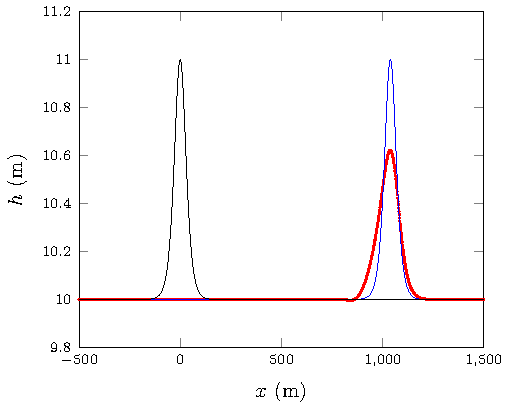
\includegraphics[width=7.0cm]{./results/soliton/ex/newo1-figure0.pdf}}
%\subfigure[][]{\label{fig:solitoneo1u}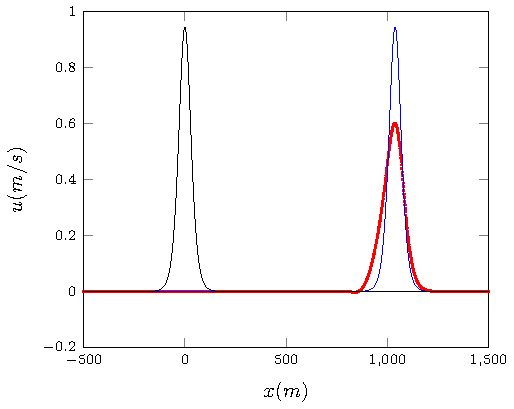
\includegraphics[width=7.0cm]{./results/soliton/ex/newo1u-figure0.pdf}}
%\subfigure[][]{\label{fig:solitoneo2h}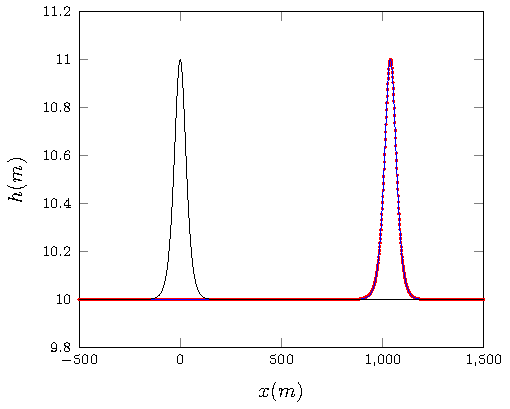
\includegraphics[width=7.0cm]{./results/soliton/ex/newo2-figure0.pdf}}
%\subfigure[][]{\label{fig:solitoneo2u}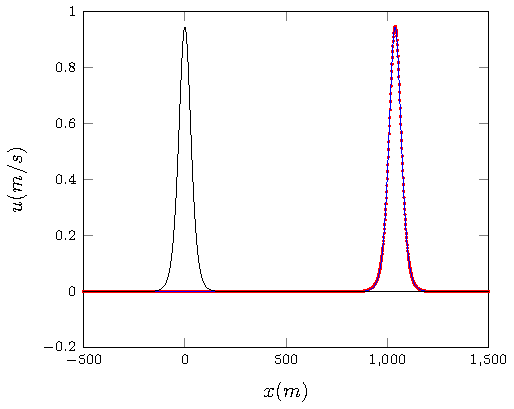
\includegraphics[width=7.0cm]{./results/soliton/ex/newo2u-figure0.pdf}}
%\subfigure[][]{\label{fig:solitoneo3h}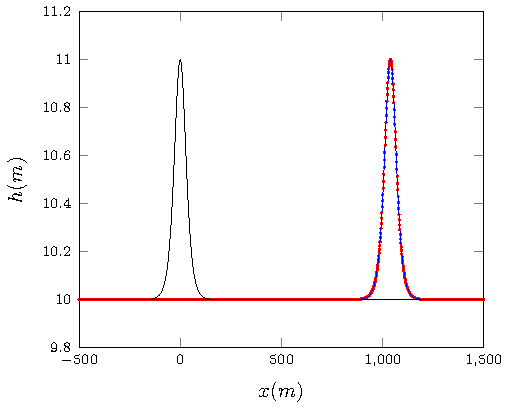
\includegraphics[width=7.0cm]{./results/soliton/ex/newo3-figure0.pdf}}
%\subfigure[][]{\label{fig:solitoneo3u}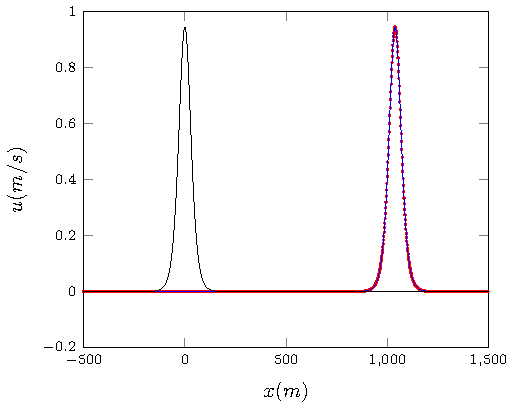
\includegraphics[width=7.0cm]{./results/soliton/ex/newo3u-figure0.pdf}}
%\caption{The first-, second- and third-order simulation of a soliton with $\Delta x = %100 /2^{6}\text{m}$ ($\circ$) plotted against the analytic solution of \eqref{eq:sol} %(\---) with black for $t =0\text{s}$ and blue for $t=100\text{s}$.}
%\label{fig:solitone}
%\end{figure}
%\begin{figure}
%\centering
%\subfigure[][]{\label{fig:solitoncono1}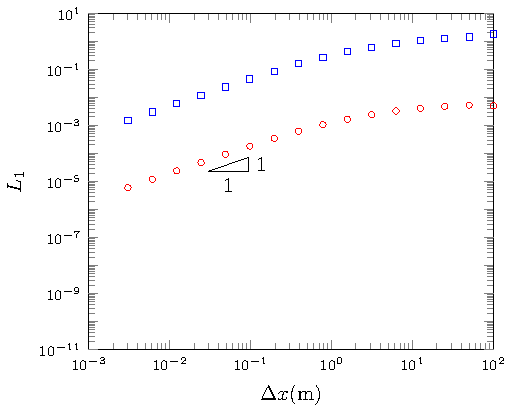
\includegraphics[width=7.0cm]{./results/soliton/con/sto1-figure0.pdf}}
%\subfigure[][]{\label{fig:solitoncono2}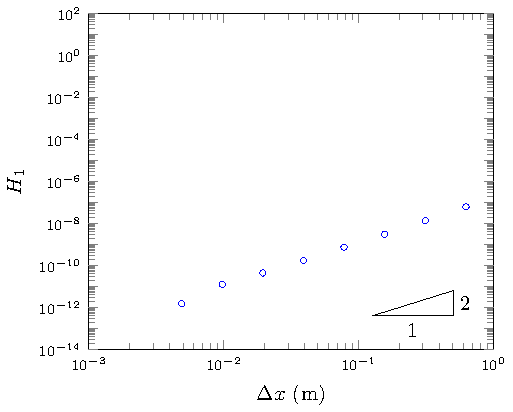
\includegraphics[width=7.0cm]{./results/soliton/con/sto2-figure0.pdf}}
%\subfigure[][]{\label{fig:solitoncono3}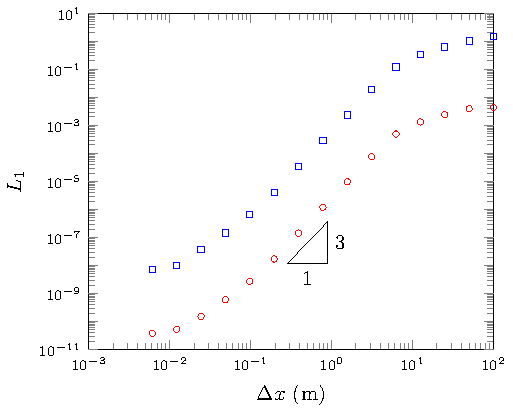
\includegraphics[width=7.0cm]{./results/soliton/con/sto3-figure0.pdf}}
%\caption{Convergence of relative error using $L_1$ norm for analytic soliton solution for both $h$ ($\circ$) and $u$ ($\diamond$) for the; (a) first-, (b) second- and (c) third-order schemes.}
%\label{fig:solitoncon}
%\end{figure} 

%Figure \ref{fig:solitone} demonstrates the superiority of the second- and third-order methods compared to the first-order method. With the first-order method there is significant attenuation of the wave due to its diffusive behaviour which creates a wider wave profile and some smaller trailing waves. However, the first-order method does produce the correct speed of the wave with a small phase error. While the second- and third-order methods demonstrate no noticeable deformation resolving the soliton solution well on a relatively coarse grid with less than $500$ cells defining the actual wave.

%The relative error as measured by the $L_1$-norm of the method can be seen in Figure \ref{fig:solitoncon}. For a vector $\boldsymbol{q}$ and an approximation to it $\boldsymbol{q}^*$ the relative error as measured by the $L_1$-norm is
%\begin{linenomath*}
%\begin{gather*}
%L_1 \left(\boldsymbol{q},\boldsymbol{q}^*\right) = \frac{\sum_{i=1}^{m} |q_i - q^*_i|}{\sum_{i=1}^{m} |q_i|}.
%\end{gather*}
%\end{linenomath*}

%Figure \ref{fig:solitoncon} demonstrates that the schemes all have the correct order of convergence in both time and space. However, this order of convergence is not uniform over all $\Delta x$. When $\Delta x$ is large the actual problem is not discretised well since the cells are too large to adequately resolve the problem; this causes the observed suboptimal rate of convergence in Figure \ref{fig:solitoncon}. When $\Delta x$ is sufficiently small the numerical errors become small enough that floating point errors are significant and this can also lead to suboptimal rates of convergence as can be seen for the third-order method in Figure \ref{fig:solitoncono3}. Therefore, the order of convergence for all methods is confirmed.

%Figure \ref{fig:solitoncon} also demonstrates the superiority of the second- and third-order schemes over the first-order scheme for accuracy. The third-order scheme is also better than the second-order scheme in this respect although this difference is less pronounced. These differences have a significant impact on run-time if one wishes to run a simulation up to a desired accuracy. For instance to run a second- or third-order scheme as accurate as the highest accuracy first-order scheme for $h$ takes significantly less time as can be seen in Table \ref{table:runtime}. This is computationally restrictive 

%Figure \ref{fig:solitoncono2} and Figure \ref{fig:solitoncono3} demonstrate that the second- and third-order schemes both have similar errors and Figure \ref{fig:solitone} shows that these schemes resolve the problem well. Therefore, the extra effort in running a third-order scheme compared to a second-order scheme is not justified in this case. While the effort required to go from a first-order to a second-order scheme is justified since attaining a similar accuracy between them requires a restrictively small $\Delta x$ for a first-order method.   

%--------------------------------------------------------------------------------
\section{Smoothed Dam-Break}
\label{section:smootheddambreak}
%--------------------------------------------------------------------------------
The discontinuous dam-break problem can be approximated by a smooth function using the hyperbolic tangent function. Such an approximation will be called a smoothed dam-break problem and will be defined as such
\begin{linenomath*}
\begin{subequations}
\begin{gather}
h(x,0) = h_0 + \frac{h_1 - h_0}{2}\left(1 + \tanh\left(\alpha\left(x_0 - x\right)\right)\right),
\end{gather}
\begin{gather}
u(x,0) = 0.0m/s.
\end{gather}
\end{subequations}
\label{eq:sdbi}
\end{linenomath*}
Where $a$ is given and controls the width of the transition between the two dam-break heights of $h_0$ and $h_1$. For large $\alpha$ the width is small and vice versa. For a fixed $\Delta x$ there are large enough $\alpha$ values such that the transition width is zero. This experiment was run for both of the methods described in this paper and the 3 different order finite difference-volume methods described in []. In this particular simulation $h_0 = 1.0m$, $h_1 = 1.8m$ on $x \in [0m,1000m]$ for $t \in [0s,30s]$ with $x_0 = 500m$. The simulations were run changing both $\Delta x$ and $\alpha$ and for stability $\Delta t = 0.01 \Delta x$ while for the second-order finite volume method $\theta = 1.2$. Since this experiment involves a very large amount of data the analysis will be broken up into three sections: decreasing $\Delta x$, increasing $\alpha$ and finally differences between the methods. 

%--------------------------------------------------------------------------------
\subsection{Changing $\Delta x$}
%--------------------------------------------------------------------------------
Decreasing $\Delta x$ allows the numerical method to better approximate the analytic solution to the equations. So for our valid [] numerical methods it would be expected that smaller $\Delta x$'s provide a closer approximation to the analytic solution This was demonstrated for smooth problems [] above.

In this comparison we pick an $\alpha$ and a method and investigate the result of decreasing $\Delta x$. Because the smoothness of the initial conditions depends on both $\Delta x$ and $\alpha$ one must be careful that the initial conditions do not change from discontinuous to smooth as $\Delta x$ is altered as then we are no longer comparing smooth problems. This is of particular importance for the two finite difference methods as they do not correctly handle discontinuos initial conditions. [] 

The first and most important observation is that there are four types of behaviour as $\Delta x \rightarrow 0$ of the problem depending on the $\alpha$ and the numerical method. It was found that the second- and third-order methods had similar $\alpha$ ranges determining the trending behaviour while the first-order had very different ranges, because of this large difference the term higher-order will be used to refer to all second- and third- order methods. Also for the purposes of simplicity these scenario's will be demonstrated by solutions of the FDVM as they are better for illustrative purposes. The four scenarios are identified by the behaviour of the solutions when $\Delta x$ is small and they correspond to different results in the literature. 

The first behaviour which will be referred to as the non-oscillatory scenario has such smooth initial conditions that there are no introduced oscillations. This scenario ends at $\alpha = 0.025$ and should in theory extend down to the trivial $\alpha = 0$, in these ranges the smoothed dam-break problem is a very poor approximation to the dam-break problem. This behaviour was observed for all methods when $\alpha = 0.025$ and an example case for the third-order method is plotted in Figure \ref{fig:o3a1dxlimflatexp}. This example demonstrates rapid convergence with all the solutions being graphically identical. This scenario resembles the solution of the shallow water wave equations in that it contains only a rarefaction and a shock with no dispersion. 

\begin{figure}
\centering
\subfigure[][]{\label{fig:o3a1dxlim}\includegraphics[width=7cm]{./results/FVMpics/1diffmdx/o3/1/nb3ne10/0-figure0.pdf}}
%\subfigure[][]{\label{fig:o3a1dxlimz1}\includegraphics[width=7cm]{./results/FVMpics/1diffmdx/o3/1/nb3ne10/1-figure0.pdf}}
\caption{Smooth dam break problem for o3 [] with $\alpha = 0.025$ for $\Delta x = 10/2^{10}$ (blue), $\Delta x = 10/2^9$ (green), $\Delta x = 10/2^8$ (red), $\Delta x = 10/2^7$ (cyan), $\Delta x = 10/2^6$ (magenta), $\Delta x = 10/2^5$ (yellow), $\Delta x = 10/2^4$ (black)}
\label{fig:o3a1dxlimflatexp}
\end{figure}

The second will be referred to as the flat scenario due to the presence of a constant height state between the oscillations at the shock and rarefaction fan. This scenario emerges at $\alpha = 0.05 $ and continues to $\alpha = 1$ for the higher-order methods and occurs from $\alpha = 0.05 $ to $\alpha = 1000 $ for the first-order method (so far). This scenario corresponds to the results presented by \citeN{Hank-etal-2010-2034} and \citeN{Mitsotakis-etal-2014}. 

An example plot demonstrating this scenario for the third-order method with $\alpha = 0.5$ can be seen in Figure \ref{fig:o3a6dxlimflatexp}. As $\Delta x$ decreases the solutions converge which is sensible since for the $\Delta x$ in Figure [] the initial conditions are smooth as can be seen in Figure [] and these methods have been verified for smooth problems. So that by $\Delta x = 10 / 2^8$ the solutions for higher $\Delta x$ are graphically identical. 

\begin{figure}
\centering
%\subfigure[][]{\label{fig:o3a6dxlim}\includegraphics[width=7cm]{./results/FVMpics/1diffmdx/o3/6/nb4ne11/0-figure0.pdf}}
\subfigure[][]{\label{fig:o3a6dxlimz1}\includegraphics[width=7cm]{./results/FVMpics/1diffmdx/o3/6/nb3ne10/0-figure0.pdf}}
\subfigure[][]{\label{fig:o3a6dxlimz2}\includegraphics[width=7cm]{./results/FVMpics/1diffmdx/o3/6/nb3ne10/1-figure0.pdf}}
\caption{Smooth dam break problem for o3 [] with $\alpha = 0.5$ for $\Delta x = 10/2^{10}$ (blue), $\Delta x = 10/2^9$ (green), $\Delta x = 10/2^8$ (red), $\Delta x = 10/2^7$ (cyan), $\Delta x = 10/2^6$ (magenta), $\Delta x = 10/2^7$ (yellow), $\Delta x = 10/2^{8}$ (black)}
\label{fig:o3a6dxlimflatexp}
\end{figure}

The third scenario will be referred to as the contact discontinuity scenario due to the use of that term to describe it by \citeN{El-etal-2006}. For the higher-order methods it occurs at $\alpha = 2.5$ and so far has not occurred for the first order method[]. The contact discontinuity scenarios main feature is that the oscillations from the rarefaction fan and the shock decay and appear to meet at a point as can be seen in Figure \ref{fig:o3a9dxlimcdexp}. For the experiments performed this doesn't appear to be an actual centre point but rather that the oscillations decay so quickly around the `contact discontinuity' that it appears to be the case. All the higher order methods so far have not shown a converged solution as $\Delta x$ decreases. However it does appear that convergence is likely with the solutions getting closer together. 

\begin{figure}
\centering
\subfigure[][]{\label{fig:o3a9dxlim}\includegraphics[width=7cm]{./results/FVMpics/1diffmdx/o3/9/nb3ne10/0-figure0.pdf}}
\subfigure[][]{\label{fig:o3a9dxlimz1}\includegraphics[width=7cm]{./results/FVMpics/1diffmdx/o3/9/nb3ne10/1-figure0.pdf}}
\subfigure[][]{\label{fig:o3a9dxlimz2}\includegraphics[width=7cm]{./results/FVMpics/1diffmdx/o3/9/nb3ne10/2-figure0.pdf}}
\caption{Smooth dam break problem for o3 [] with $\alpha = 2.5$ for $\Delta x = 10/2^{10}$ (blue), $\Delta x = 10/2^9$ (green), $\Delta x = 10/2^8$ (red), $\Delta x = 10/2^7$ (cyan), $\Delta x = 10/2^6$ (magenta), $\Delta x = 10/2^5$ (yellow), $\Delta x = 10/2^{4}$ (black)}
\label{fig:o3a9dxlimcdexp}
\end{figure}

The fourth scenario will be referred to as the bump scenario due to the oscillations no longer decaying down towards a point but rather growing around where the contact discontinuity was in the previous scenario as can be seen in Figure \ref{fig:o3a20dxlimcdexp}. This behaviour has hitherto not been presented and is certainly not an expected result. There are some important observations, changing $\alpha$ does increase the height of the bump for the lowest resolution methods although after [] increasing $\alpha$ has no effect[huh?]. The behaviour of these solutions in Figure \ref{fig:o3a20dxlimcdexp} do not clearly show convergence, although it doesn't appear that there is a rapid divergence which suggests that this behaviour is not unstable. Also the lack of convergence is only around the contact discontinuity with other parts of the solution showing convergence. 

\begin{figure}
\centering
\subfigure[][]{\label{fig:o3a20dxlim}\includegraphics[width=7cm]{./results/FVMpics/1diffmdx/o3/20/nb3ne10/0-figure0.pdf}}
\subfigure[][]{\label{fig:o3a20dxlimz1}\includegraphics[width=7cm]{./results/FVMpics/1diffmdx/o3/20/nb3ne10/1-figure0.pdf}}
\subfigure[][]{\label{fig:o3a20dxlimz2}\includegraphics[width=7cm]{./results/FVMpics/1diffmdx/o3/20/nb3ne10/2-figure0.pdf}}
%\subfigure[][]{\label{fig:o3a20dxlimz3}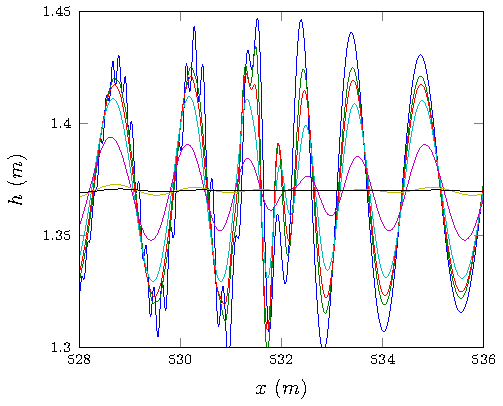
\includegraphics[width=7cm]{./results/FVMpics/1diffmdx/o3/20/nb3ne10/4-figure0.pdf}}
\caption{Smooth dam break problem for o3 [] with $\alpha = 1000.0$ for $\Delta x = 10/2^{10}$ (blue), $\Delta x = 10/2^9$ (green), $\Delta x = 10/2^8$ (red), $\Delta x = 10/2^7$ (cyan), $\Delta x = 10/2^6$ (magenta), $\Delta x = 10/2^7$ (yellow), $\Delta x = 10/2^{8}$ (black)}
\label{fig:o3a20dxlimcdexp}
\end{figure}

All of the scenarios described above and displayed using the higher-order FDVM also occur for the FDM, however because finite differences cannot properly handle discontinuities this is a little more subtle. Firstly, since for each $\alpha$ there is a $\Delta x$ such that for larger $\Delta x$ the smooth dam break problem is no longer smooth enough for a finite difference approximation to be appropriate. This becomes a problem for the contact discontinuity and bump scenarios since they require higher $\alpha$ and are thus more discontinuous to begin with. The result of this are non-physcial looking oscillations for large $\Delta x$ values that were not replicated by the FDVM and thus can be attributed to this flaw of FDM as in Figure []. 

Overall there where two types of trending behaviours as $\Delta x$ was decreased one for the FDM and another for the FDVM. FDM decreased the number of oscillations in the solution as in Figure [], while FDVM increased the number of oscillations in the solution as can be seen in Figure []. This is explained by \citeN{Zoppou-Roberts-1996} as the FDM are second order finite difference approximations their errors are dissipative thus introducing oscillatory errors which are most prominent when $\Delta x$ and therefore the errors are large. While the behaviour of the FDVM is explained by a series of effects [] [TVD, treating things as cell averages, thus flattening things in cells,]. 

 

[](verify convergence rates near discontinuities?) 

%--------------------------------------------------------------------------------
\subsection{Changing $\alpha$}
%--------------------------------------------------------------------------------
Increasing $\alpha$ allows the initial conditions \eqref{eq:sdbi} to approach the dam break problem with $h_1$ to the left and $h_0$ to the right centred around $x_0$. So it would be expected that as $\alpha \rightarrow \infty$ that the solution of the smooth dam break problem would approach the corresponding dam break problem. This is the case for numerical methods because for a fixed $\Delta x$ $\alpha$ can be chosen large enough that \eqref{eq:sdbi} is precisely the dam break problem. This can be seen in Figure [] with $\Delta x =$ where the required $\alpha$ for this to occur is below $1000$ which was the maximum $\alpha$ value used in these experiments. However, only the FDVM were able to handle such large $\alpha$'s because the initial conditions are not smooth enough to allow for stability in the FDM as can be seen in Figure []. While the FDVM handled this quite well and for all $\Delta x$ tested as $\alpha$ increased the solutions converged, even though for higher $\Delta x$ [] $\alpha$ was not large enough to make \eqref{eq:sdbi} a jump discontinuity. 

This confirms the superiority of the FDVM to handle non smooth initial conditions and the inability of FDM to handle them. Even near discontinuous initial conditions caused problems for the FDM with the introduction of oscillations that were not replicated by the FDVM and appeared to be non-physical. An example of these transitional solutions between the properly smooth initial conditions and the unstable discontinuous ones can be seen in Figure []. [](only compare the models when FD started smooth enough)

For the range of $\alpha$'s which are smooth enough for the FDM to be appropriate then as $\alpha$ increases the number of oscillations increases as well for both the FDM and the FDVM. So that the smoothness of the initial conditions controls the oscillations but this depends on $\Delta x$ since for a fixed $\alpha$ the smoothness of the discretised initial conditions depends on $\Delta x$. [] (relative smoothness, more universal number)

It was observed that $\Delta x$ can be chosen large enough such that increasing $\alpha$ does not resolve some of the more complex structure observed for smaller $\Delta x$ values. This $\Delta x$ depends on the model most notably for the first-order finite difference-volume scheme this $\Delta x$ is very small. An example of this for the third-order FDVM scheme can be seen in Figure []. 



%--------------------------------------------------------------------------------
\subsection{Comparison of Models}
%--------------------------------------------------------------------------------
The first-order FDVM was too diffuse and


%\subsection{Dam-Break} %old
%--------------------------------------------------------------------------------
%The dam-break problem can be defined as such
%\begin{linenomath*}
%\begin{gather*}
%h(x,0) = \left\lbrace \begin{array}{c c}
%1.8 & x < 500\\
%1.0 & x \ge 500\\
%\end{array} \right. ,
%\end{gather*}
%\begin{gather*}
%u(x,0) = 0.0m/s.
%\end{gather*}
%\end{linenomath*}
%With $x \in \left[0\text{m},1000\text{m}\right]$ for $t \in \left[0\text{s},30\text{s}\right]$. Where $\lambda = 0.01 \text{m/s}$ and $\theta = 1.2$. This corresponds to sub-critical flow and was a situation demonstrated in \citeN{El-etal-2006} and \citeN{Hank-etal-2010-2034}. An example was plotted for %$\Delta x = 100 /2^{10}\text{m}$ for all the methods and for $\Delta x = 100 %/2^{15}\text{m}$ for the first-order method in Figure \ref{fig:DB}. To determine if %the oscillations that occur in the solution indeed converge to some limit as $\Delta x %\rightarrow 0$ multiple $\Delta x$ values were run and then the amount of variation in %the solution measured. This measured how oscillatory the solution was and was used to %determine the growth of the oscillations. A common way to measure this is the total %variation $TV$ \cite{LeVeque-2002} which for $\boldsymbol{q}$ is given by
%\begin{linenomath*}
%\begin{gather*}
%TV(\boldsymbol{q}) = \sum_{\forall i >1} |q_{i} - q_{i-1}|.
%\end{gather*}
%\end{linenomath*}
%If the solution does indeed converge then the TV must at some point plateau, bounding the oscillations. This was indeed the findings of the experiments as can be seen by Figure \ref{fig:DBL1}. The TV increases as $\Delta x$ decreased because the models resolved more dispersive waves. As $\Delta x$ decreased further the TV plateaued and so the size and number of oscillations was bounded. Therefore, the scheme has not become unstable which supports the argument that the numerical schemes do not introduce non-physical oscillations in the solution. The second-order scheme converges rapidly to the solution of the third-order scheme.

%\begin{figure}
%\begin{center}
%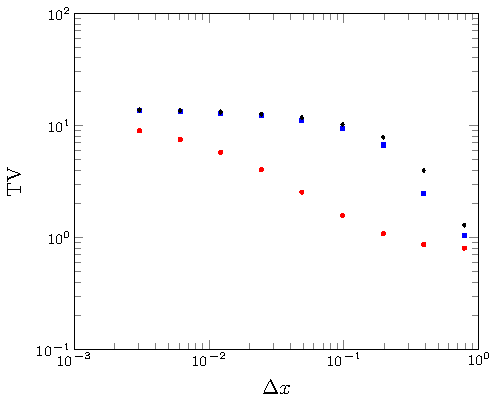
\includegraphics[width=8.0cm]{./results/dambreak/L1con/both-figure0.pdf}
%\end{center}
%\caption{The change in total variation (TV) over $\Delta x$ for; ($\circ$) first- , %($\square$) second-, and ($*$) third-order schemes.}
%\label{fig:DBL1}
%\end{figure}
%\begin{figure}
%\centering
%\subfigure[][]{\label{fig:DBo1}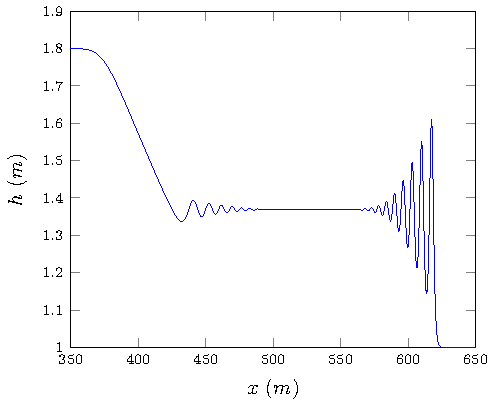
\includegraphics[width=7cm]{./results/dambreak/ex/o1-figure0.pdf}}
%\subfigure[][]{\label{fig:DBo2}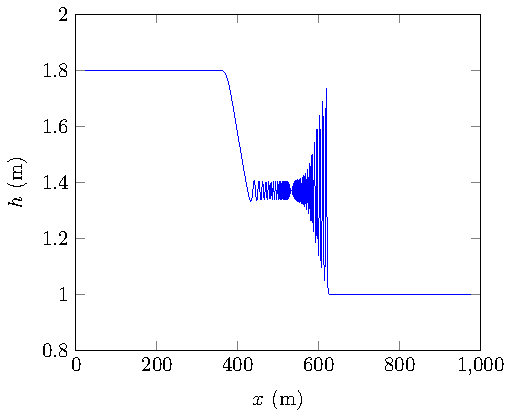
\includegraphics[width=7cm]{./results/dambreak/ex/o2-figure0.pdf}}
%\subfigure[][]{\label{fig:DBo3}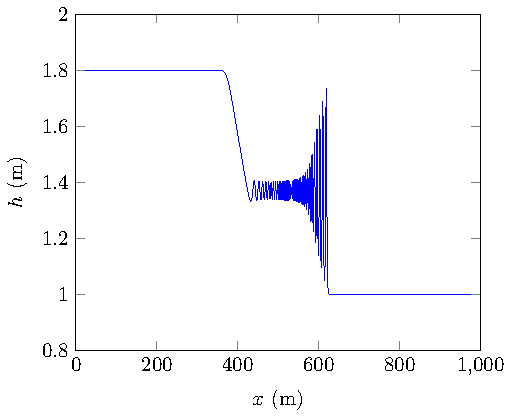
\includegraphics[width=7cm]{./results/dambreak/ex/o3-figure0.pdf}}
%\subfigure[][]{\label{fig:DB1o1}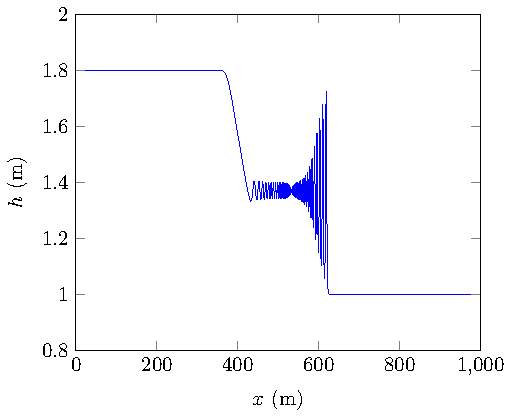
\includegraphics[width=7cm]{./results/dambreak/ex/o1-figure1.pdf}}
%\caption{Solution of the dam-break problem using the (a) first-, (b) second- and (c) third-order method with $\Delta x = 100 /2^{10} \text{m}$. As well as a (d) first-order method with $\Delta x = 100 /2^{15} \text{m}$. }
%\label{fig:DB}
%\end{figure}

%These solutions compare very well to the findings in \citeN{El-etal-2006} with both the second- and third-order schemes resolving the oscillations around the "contact discontinuity"\cite{El-etal-2006} between the rarefaction fan and the shock. In \citeN{Hank-etal-2010-2034} it was reported that for their first-order scheme such oscillatory behaviour was not seen. However, for the first-order scheme proposed in this paper when $\Delta x = 100 /2^{15}$ it was resolved as in Figure \ref{fig:DB1o1}. This validates the findings in \citeN{El-etal-2006}.

%There is also a good agreement between the second- and third-order simulations of the dam-break problem as can be seen in Figures \ref{fig:DBo2} and \ref{fig:DBo3}. Although more oscillations are resolved by the third-order scheme over the second-order scheme, there is no significant change in the resolved behaviour of this problem between the two schemes. As noted in the introduction second-order errors are dissipative; since the diffusive third-order scheme resolved the same oscillations it was demonstrated that none of the dissipative errors significantly polluted the wave train and so the second-order scheme is capable of resolving the problem well.
%--------------------------------------------------------------------------------
\section{Conclusions}
\label{section:Conclusions}
%--------------------------------------------------------------------------------

%--------------------------------------------------------------------------------
\section{Acknowledgements}
%--------------------------------------------------------------------------------

%--------------------------------------------------------------------------------
\bibliography{Serre_ASCE}
%--------------------------------------------------------------------------------

\end{document}
